\TUchapter{Evaluation}

This chapter presents the evaluation of \textit{JPF-SymSpark} in two dimensions: a qualitative appraisal of the overall tool and a quantitative performance assessment of iterative symbolic executions. Additionally, the chapter concludes with a discussion of the limitations of the tool and its processes. 

The qualitative appraisal aims to contrast \textit{JPF-SymSpark} against a series of functional requirements of an ideal symbolic execution framework for Apache Spark. The performance assessment of the iterative symbolic executions explores the behavior of the iterative reduce strategy in order to highlight performance obstacles when choosing this execution approach. Lastly, the discussion on the limitations provides additional information on the constraints, for both the tool and the process, under the context of \jpf{}.

%The next sections are structured as follows: First, the requirements for an ideal symbolic execution tool for Spark programs are enunciated. Next, \textit{JPF-SymSpark} is contrasted against each of the defined requirements in order to determine if they are met. Additionally, the performance evaluation of the iterative reduce strategy is presented. Finally, the limitations of \textit{JPF-SymSpark} and the whole \acrshort{acr:jpf} framework are discussed.

\TUsection{Qualitative Evaluation}
\label{sec:qualitative}

For the qualitative examination, we specify a series of conceptual requirements that define the functionality of an ideal tool used to conduct symbolic executions on Spark programs. \textit{JPF-SymSpark} is then compared against these requirements in order to determine how successful the implementation of the module is. Given that, to our knowledge, \textit{JPF-SymSpark} is the only tool capable of carrying out symbolic executions on a big data framework, it is relevant to identify what are the main requirements for a tool with such a goal in order to define a complying criteria for further evaluations.

The purpose of this evaluation is to respond some of the research questions stated in Chapter~1. In particular, the requirements elaborate the aim further, offering a detailed description of what means to conduct symbolic executions on Spark programs. Additionally, the requirements answer directly to the second research question ---\textit{What are the particular characteristics associated with the symbolic execution of a Spark program?} while the evaluation of \textit{JPF-SymSpark} also aims to answer the fourth research question, specifically regarding \spf{} ---\textit{What are the advantages and disadvantages of such a framework in the context of Spark applications?}

The requirements presented in this section are as generic as possible, without falling into the specifics of any architecture or programming language. They focus on the capacity of generating artificial input values that ensure full path coverage, which is the ultimate goal of this research work. The following list presents the nine identified requirements and also provides a brief explanation for each of them. 

\TUsubsection{Requirements}
\label{sec:requirement}

\newcommand{\reqitem}[1]{\item[\textit{\textbf{R.#1}}]}
\begin{itemize}
\reqitem{1} \textit{The framework should produce a reduced input dataset that ensures full path coverage of the program under test}

This is the core requirement for such a framework. The expected output of a symbolic execution should be a dataset with as few elements as possible that can be used as input in a regular run of the program under test to ensure full path coverage. There could be several use cases for such an input dataset, for example, the generation of automated unit tests that assert the correct termination of the program.

\reqitem{2} \textit{The framework should report unfeasible path conditions in case there are any}

Unfeasible paths are a sign of faulty implementations or wrong design assumptions. It is highly desirable that the framework notifies when an unfeasible path is found because such information will aid developers to focus on flawed portions of the source code.

\reqitem{3} \textit{The framework shall conduct a symbolic execution of all the operations that conform the program, ensuring the correct interconnection between consecutive transformations and actions}

A holistic analysis of a Spark program is only reasonable if intra-procedural and inter-procedural evaluation are ensured. Conducting symbolic executions on each relevant operation independently is not sufficient to argue on the whole data flow. For this reason, ensuring the right propagation of symbolic values among operations is crucial for a significant analysis.
	
\reqitem{4} \textit{The framework shall conduct a symbolic execution of the program under test without requiring any modification to its source code}

Black-box approaches promote the adoption of the analysis tool and ensure that the program under test is faithfully a representation of a real program. Additionally, such approaches could be integrated with developer environments in order to conduct automated analyses and provide suggestions in real-time, whereas this could not be possible if the tool would require the manipulation of the source code. 
	
\reqitem{5} \textit{The framework shall be able to reason over symbolic primitive types}

Primitive types represented as their respective wrappers classes in Java should be supported. Symbolic path conditions for these types are often represented as linear and non-linear arithmetical equations. However, few Spark programs work solely on \acrshort{acr:rdd}s of simple primitive types, more elaborate data structures are used often.
	
\reqitem{6} \textit{The framework shall be able to reason over symbolic Strings}

Spark is frequently used to process large amounts of text input, usually in the form of whole files. One example of such an algorithm is the calculation of an inverted index, used commonly in search engines to map key terms to the document where they are found. For this reason, supporting symbolic String operations is fundamental for such a framework.
	
\reqitem{7} \textit{The framework shall be able to reason over symbolic data structures}

In a similar form, many Spark programs work on more complex data structures. Tuples in particular are widely used, having even in some cases specific operations defined on them, such is the case of \textit{reduceByKey}.
	
\reqitem{8} \textit{The framework should support all Spark programs that compile correctly}

A valid Spark program should always be supported even if there is no relevant dataset to be inferred. This enforces the usability of the framework.
	
\reqitem{9} \textit{The framework shall be able to process iterative and cumulative actions}

Some Spark actions, such as \textit{reduce}, have an iterative behavior over the elements of an \acrshort{acr:rdd}. In some cases an accumulated value could participate in branching operations; this causes the path conditions to change for every element processed. The framework should be able to reason about how this path conditions will change after every iteration and provide different input datasets that explore their respective paths based on how many elements they contained.

\end{itemize}

These general requirements are sufficient to describe a tool for the symbolic execution of Spark program by dealing with the specific conditions of the big data framework. Further studies can use and extend these primary requirements to conduct additional evaluations to other data intensive frameworks. 

\TUsubsection{Validation}

For the validation, each requirement introduced in Section~\ref{sec:requirement} is revisited and discussed in the context of \textit{JPF-SymSpark}. We indicate first whether \textit{JPF-SymSpark} complies or not with the requirement and, subsequently, provide an explanation on how this was concluded. On occasions, requirements are only partially met, in which case the reasons for a partial fulfillment are explained. However, Section~\ref{sec:limitations} offers a thorough discussion of the limitations of the tool. Moreover, Table~\ref{tab:evaluation:quantitative} presents a summary of the validation results.

\begin{itemize}
\reqitem{1} \textit{The framework should produce a reduced input dataset that ensures full path coverage of the program under test}

This requirement is fulfilled. As explained in Section~\ref{subsec:module:output}, \textit{JPF-SymSpark} produces two types of output as a consequence of the symbolic execution. The first is a single input dataset containing a value for each satisfiable path condition found. This dataset is, in fact, minimal given that only one value per path condition is taken. The second type is a family of input datasets produced as a consequence of the symbolic execution of iterative aggregate operations. In this case, all the elements in a dataset follow the same single path condition until they are combined in the aggregate operation. Moreover, the cardinality of the datasets indicates the number of iterations considered in the analysis.

Certifying that the generated datasets actually ensured full path coverage comes as a direct consequence on how the elements of the dataset were obtained. However, we used \textit{JaCoCo}~\cite{JaCoCo2017}, a code coverage analysis tool for Java programs that is capable of measuring different levels of coverage in order to verify the assumption in several examples. Although there is no tool for the Java programming language that is capable of measuring path coverage, \textit{JaCoCo} is able to measure branch coverage and cyclomatic complexity~\cite{McCabe1976} (only intra-procedural), which gives an approximation to path coverage metrics. In all the evaluated examples, the obtained datasets offered full coverage in the two aforementioned metrics.

\reqitem{2} \textit{The framework should report unfeasible path conditions in case there are any}

This requirement is fulfilled. Again, as explained in Section~\ref{subsec:module:output}, \textit{JPF-SymSpark} reports unfeasible path conditions as soon as they are found.

\reqitem{3} \textit{The framework shall conduct a symbolic execution of all the operations that conform the program, ensuring the correct interconnection between consecutive transformations and actions}

This requirement is fulfilled. The main contribution of \textit{JPF-SymSpark} is to provide a framework that allows the symbolic execution of consecutive Spark operations by correctly connecting the respective input and output values of each operation. This approach allows a comprehensive analysis of a program instead of a method-by-method reasoning.

\reqitem{4} \textit{The framework shall conduct a symbolic execution of the program under test without requiring any modification to its source code}

This requirement is fulfilled. \textit{JPF-SymSpark} was designed to work as a black-box tool. The surrogate Spark library is only included in the \jpf{}'s classpath as it is specified in the corresponding \textit{.properties} file, making it only available during the analyses. Normal executions of the program under test do not include the surrogate library, using instead the official Spark library.

\reqitem{5} \textit{The framework shall be able to reason over symbolic primitive types}

This requirement is fulfilled. Spark operations over \acrshort{acr:rdd}s of \textit{Integer}, \textit{Long}, \textit{Float}, \textit{Double} and \textit{Boolean} wrapper classes are supported.

\reqitem{6} \textit{The framework shall be able to reason over symbolic Strings}

This requirement is partially fulfilled. Support on symbolic String operations is constrained by the limitations of \spf{}. This poses a major limitation for the adoption of the tool given that many big data tasks rely on text processing. More on this in Section~\ref{sec:limitations}.

\reqitem{7} \textit{The framework shall be able to reason over symbolic data structures}

This requirement is not fulfilled. Support to symbolic data structures in \spf{} is faulty; as a consequence, \textit{JPF-SymSpark} is not capable of reasoning on \acrshort{acr:rdd}s of any complex data structures. This represents a major limitation given that Tuples are frequently used in big data tasks to group data.

\reqitem{8} \textit{The framework should support all Spark programs that compile correctly}

This requirements is partially fulfilled. \textit{JPF-SymSpark} relies on a surrogate Apache Spark library that is used for two purposes: First, to relief \jpf{} from processing irrelevant operations for a symbolic execution, such as context initialization. The second, simplify the methods in the \acrshort{acr:rdd}'s API in order to facilitate the symbolic executions, for example, removing loops and additional considerations relative to distributed computing. This library is not exhaustive, for this reason, there will be unsupported operations that compile under the regular Spark library. Furthermore, other Spark APIs, such as the Dataset API, are not supported.

\reqitem{9} \textit{The framework shall be able to process iterative and cumulative actions}

This requirement is partially fulfilled. Only actions that work on primitive values are supported. As a consequence of \textit{R.7}, all the actions that work on symbolic data structures cannot be processed. Moreover, the symbolic output of aggregate functions is not percolated beyond the boundaries of the operation; this means that any branching condition applied on the return value of an action is not symbolically executed.
\end{itemize}

\begin{table}[t]
	\centering
	\large
	\begin{tabular*}{0.8\textwidth}{@{\extracolsep{\fill}}lcccccccccc}
		& R.1 & R.2 & R.3 & R.4 & R.5 & R.6 & R.7 & R.8 & R.9 \\
		\hline
		\rule{0pt}{2.5ex}
		\textit{JPF-SymSpark} & \checkmark & \checkmark & \checkmark & \checkmark & \checkmark & \dag & \texttimes & \dag & \dag \\
		\hline
	\end{tabular*}
	\caption*{		
		\begin{tabular}{l l l l l l}
			\footnotesize{Fulfilled} & $\checkmark$ & \footnotesize{Not fulfilled} & $\times$ & \footnotesize{Partially fulfilled} & $\dag$ \\
		\end{tabular}
	}
	\caption[Summary of the Qualitative Validation of \textit{JPF-SymSpark}]{Summary of the qualitative validation of \textit{JPF-SymSpark}.}
	\label{tab:evaluation:quantitative}
\end{table}

Although most of the requirements are met, those that are only partially met or not met at all represent severe obstacles to the applicability of the tool on less trivial Spark programs. With the exception of requirement \textit{R.8}, the rest of the requirements that are not fully met are obstructed by limitations of the underlying tools and frameworks used to conduct the analysis. Improving the symbolic execution framework and the constraint solvers is mandatory for the fulfillment of all the defined requirements. Nevertheless, the proposed process and the foundation of \textit{JPF-SymSpark} lay the ground for further research on this topic.
\TUsection{Quantitative Evaluation of Iterative Symbolic Executions}

The process carried out by the iterative reduce strategy resembles a loop unwinding technique, where an iterative behavior is taken out of a loop and executed sequentially without the need of accumulators or counters. This approach is often used to improve the execution speed of a program by getting rid of all the control flow instructions inherent to loop statements. However, regarding \textit{JPF-SymSpark} and several other program analysis techniques, loop unwinding is used to bound the execution of potentially infinite loop instructions, hence allowing the evaluation of the program under test.

\textit{JPF-SymSpark} allows the user to specify the number of iterations of an aggregated function that will be symbolically executed. This enables the module to bound the execution of the iterative behavior and carry out the analysis by correctly chaining the outcome of previous iterations. However, the number of path conditions grow exponentially with the number of conditional statements found. This means that if the aggregate function being analyzed has a conditional statement, then it is most likely that a path explosion will occur.

This evaluation focuses on the behavior of the iterative reduce strategy and it aims to identify the major aspects that pose performance losses. It illustrates how an increment in the number of iterations to be considered in the analysis has a direct impact on the number and size of path conditions, as well as in the performance of the constraint solvers. Moreover, it serves as an example to identify path explosion in symbolic executions.

\TUsubsection{Setup}

Four scenarios were considered for the experiments:

\begin{itemize}
	\item \textbf{Iterative Reduce with Non-Cumulative Condition (IRNC)}: The program under test contains a single \textit{reduce} action with a conditional instruction defined only over a non cumulative symbolic variable.
	\item \textbf{Iterative Reduce with Cumulative Condition (IRC)}: Also a single \textit{reduce} action but this time the conditional instruction is defined over the cumulative symbolic variable.
	\item \textbf{Iterative Map and Reduce with Non-Cumulative Condition (IMRNC)}: This scenario is similar to the first one with the difference that the \textit{reduce} action is preceded by a \textit{map} transformation with a single conditional statement over its symbolical variable.
	\item \textbf{Iterative Map and Reduce with Cumulative Condition (IMRC)}: Same as the previous scenario except that the \textit{reduce} action has a conditional instruction defined over its cumulative symbolic variable.
\end{itemize}

The first two scenarios aim to determine what kind of performance effects generate from solving constraints based on cumulative and non cumulative constraints. The last two scenarios are used to measure the relevance of previous transformations that manipulate the symbolic variable and also introduce a condition to the path before the \textit{reduce} action. All the scenarios were implemented as trivial Spark programs processing only integer values. Furthermore, the conditional statements between operations were defined in a way that unsatisfiable path conditions would be generated eventually.

Each scenario was executed for 2, 3, 5, 8 and 13 iterations respectively, repeating each case ten times and taking the average of the execution time as the result. This range follows a Fibonacci sequence and was chosen to space out the iterations enough to make any trend distinguishable. Additionally, for each case, the number of satisfiable and unsatisfiable path conditions was registered. The experiments were carried out in a laptop computer with an Intel Core-i7-6500U processor at 2.50GHz and assigning 1GB of memory to the JVM executing the analysis. \jpf{} was triggered using the command line instead of the Eclipse JPF plugin in order to avoid wasting memory in processes inherent to the Eclipse IDE.

\TUsubsection{Results and Discussion}

The results of the experiments are summarized in Table~\ref{tab:evaluation:quantitative-time} for the executions times, and in Table~\ref{tab:evaluation:quantitative-path-conditions} for the number of satisfiable and unsatisfiable path condition for each scenario.

\textbf{Execution times}

All the scenarios have a similar performance up until three symbolic iterations. However, the performance of some scenarios starts to diverge after five iterations. The starkest difference is displayed by the \textit{IRC} scenario, where the execution times increase several orders of magnitude in comparison to the other scenarios. In particular, the \textit{IRC} scenario could not be executed for 13 iterations or more, resulting in executions that lasted several hours and culminating eventually in \textit{OutOfMemory} exceptions.

The rest of the scenarios have a steady increase in their measurements until they reach 13 symbolic iterations, where the execution times start to grow exponentially. From the remaining three scenarios, the \textit{IMRC} scenario displays the worst performance, taking almost three minutes to execute 13 symbolic executions. Figure~\ref{fig:evaluation:quantitative} presents a plot of the execution times in a logarithmic scale that better depicts the disparity between some of the scenarios.

\begin{table}[t]
	\centering
	\small
	\begin{tabular*}{0.9\textwidth}{@{\extracolsep{\fill}} lccccc}
		\hline
		Iterations & 2 & 3 & 5 & 8 & 13 \\
		\hline\hline
		IRNC  & 0.680 & 0.705 & 0.855  & 1.344   & 5.489   \\
		IRC   & 0.589 & 0.625 & 15.616 & 568.004 & N/A      \\
		IMRNC & 0.669 & 0.710 & 0.981  & 2.621   & 21.662  \\
		IMRC  & 0.681 & 0.728 & 1.144  & 2.585    & 177.579 \\
		\hline	
	\end{tabular*}	
	\caption[Average Execution Times]{Average execution time in seconds for each scenario under the different number of executed iterations.}
	\label{tab:evaluation:quantitative-time}
\end{table}

\begin{figure}
	\centering	
	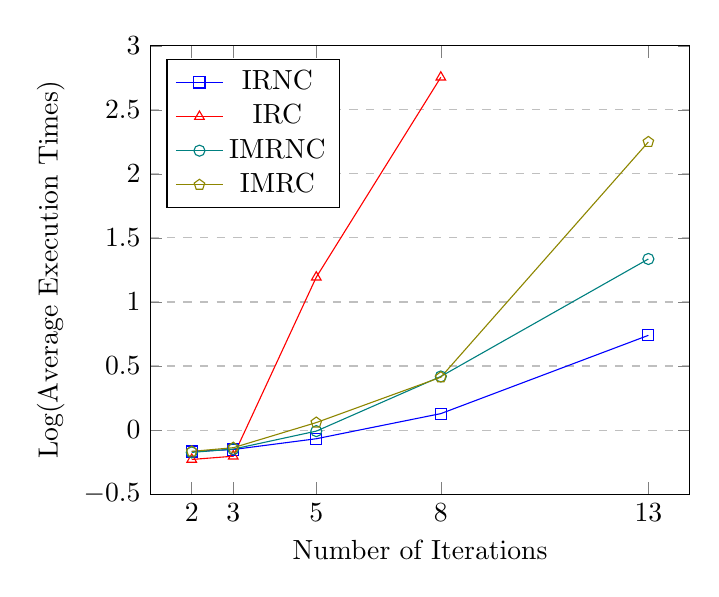
\begin{tikzpicture}
		\begin{axis}[
%			title={Average Execution Times in Log10},
			xlabel={Number of Iterations},
			ylabel={Log(Average Execution Times)},
			xmin=1, xmax=14,
			ymin=-0.5, ymax=3,
			xtick={2,3,5,8,13},
			ytick={-0.5,0,0.5,1,1.5,2,2.5,3},
			legend pos=north west,
			ymajorgrids=true,
			grid style=dashed,
		]
			
			\addplot[
			color=blue,
			mark=square,
			]
			coordinates {
				(2,-0.1673633724)(3,-0.151810883)(5,-0.0676277179)(8,0.1284638911)(13,0.739524878)
			};
	
			\addplot[
			color=red,
			mark=triangle,
			]
			coordinates {
				(2,-0.2294425251)(3,-0.2040505011)(5,1.1935725814)(8,2.7543517764)
			};
			
			\addplot[
			color=teal,
			mark=o,
			]
			coordinates {
				(2,-0.1741197011)(3,-0.148619332)(5,-0.0081539464)(8,0.4185829941)(13,1.3357165949)
			};
			
			\addplot[
			color=olive,
			mark=pentagon,
			]
			coordinates {
				(2,-0.1663430031)(3,-0.1376300629)(5,0.058615797)(8,0.4124605474)(13,2.2493920951)
			};
	
			\legend{IRNC, IRC, IMRNC, IMRC}
		\end{axis}
	\end{tikzpicture}
	\caption[Average Execution Times in Logarithmic Scale]{Average execution times in logarithmic scale. The disparity between the scenarios is easily perceived using a logarithmic scale while still preserving the notion of exponential growth.}
	\label{fig:evaluation:quantitative}
\end{figure}


\textbf{Number of path conditions}

As expected, the total number of path conditions grows exponentially over the number of iterations executed. The scenarios having a \textit{map} transformation before the iterative action have double the total amount of path conditions than their counterparts without the transformation. This is consistent with the exponential growth of the number of path conditions given that the transformation only introduced an additional branching statement.

Nevertheless, the number of unsatisfiable path conditions varies strongly depending on the scenario being studied. In the case of the \textit{IRNC} scenario, all path conditions are satisfiable, while for the \textit{IRC} scenario, only a few in the case of 8 iterations are not satisfiable; most of these resulting from timeouts of the constraint solvers. On the contrary, the \textit{IMRNC} and \textit{IMRC} scenarios present high rates of unsatisfiable path conditions throughout the different number of iterations, ranging from 30\% to 50\% for the former and from 45\% to 90\% for the latter.

\textbf{Discussion}

The results obtained in these experiments highlight some key features of the behavior of symbolic execution applied to aggregate functions. First, the performance of the framework is considerably better when the conditional statements defined in the aggregate function only affect the non-cumulative symbolic variable in the operation. This comes as a consequence of the kind of constraints generated in such cases. In the case of non-cumulative conditions, the constraints are defined over single independent symbolic variables that are joined in a conjunction on each iteration, while in the case of cumulative conditions, after each iteration, the constraints include more symbolic variables related with each other. Constraint solvers perform better when the constraints are defined over independent symbolic variables, which explains the behavior of the \textit{IRC} scenario and the difference between the cumulative and non-cumulative scenarios in general.

Another aspect is the difference between the \textit{IRC} and \textit{IMRC} scenarios. After five iterations, the behavior of these two scenarios strongly diverge, having the \textit{IRC} scenario performing exponentially worse and even reaching the point of not being able to finish its execution, while the \textit{IMRC} scenario is still capable to finish the execution within a reasonable amount of time. This is due the number of unsatisfiable path conditions in the \textit{IMRC} scenario because, although this scenario has more path conditions than the \textit{IRC} scenario, a large number of them are unsatisfiable, allowing the constraint solver to conclude faster. This result indicates that having more path conditions does not necessarily translates into worse performance; it depends on how complex the path conditions are and how many of them are actually satisfiable.

The performance of the constraint solver, as well as the complexity of the path conditions, are the major factors that affect the overall performance of iterative symbolic executions in \textit{JPF-SymSpark}. Moreover, the construction of aggregate functions with conditional statements has to be properly evaluated in terms of the congruency of the operation. Conditions applied to a cumulative value can break the associativity requirement of reducer functions, leading to invalid, non-parallelizable Spark programs.

\begin{table}[t]
	\centering
	\small
	\begin{tabular*}{0.9\textwidth}{@{\extracolsep{\fill}} lcc|cc|cc|cc|cc}
		\hline
		Iterations & \multicolumn{2}{c}{2} & \multicolumn{2}{c}{3} & \multicolumn{2}{c}{5} & \multicolumn{2}{c}{8} & \multicolumn{2}{c}{13} \\
		&  s & u & s & u & s & u & s & u & s & u \\		
		\hline\hline
		IRNC   & 6 & 0 & 14 & 0  & 62 & 0  & 510 & 0   & 16382 & 0     \\
		IRC    & 6 & 0 & 14 & 0  & 62 & 0  & 454 & 56  & n/a & n/a     \\
		IMRNC  & 8 & 4 & 17 & 11 & 67 & 57 & 518 & 512 & 16395 & 16369 \\
		IMRC   & 7 & 5 & 12 & 16 & 25 & 99 & 57  & 963 & 573   & 32191 \\
		\hline	
	\end{tabular*}
	\caption[Number of Satisfiable and Unsatisfiable Path Conditions]{Number of satisfiable and unsatisfiable path conditions for each scenario under the different number of executed iterations. As a reference, the letter ``s'' stands for satisfiable while the letter ``u'' stands for unsatisfiable.}
	\label{tab:evaluation:quantitative-path-conditions}
\end{table} 
\TUsection{Limitations}
\label{sec:limitations}

%Mention how JPF-SymSpark is limited in terms of the fixed Spark library that it checks and the Java-only compatibility
%
%The limited support to String symbolic operations. The lack of a solver that specializes on Strings makes it limited to supporting many big data tasks.
%
%Limited support to objects and how symbolic objects are created and shared
%
%The ugly ill-maintained codebase of jpf-symbc makes it cumbersome to extend and easily outdated due to abundance of code smells and bad practices.
%
%The complications when dealing with lambda expressions makes it difficult to use the tool on real spark applications. Because most current developers prefer java8 syntax favoring its flexibility and reduced verbosity.
%
%Although support for other solvers is mentioned, in practice, many of them fail due to missing libraries which are outdated when independently included.

This section comments on several limitations of \textit{JPF-SymSpark} that come as a direct consequence of the design decisions or are caused by any of the frameworks upon which the module builds up.

The processing logic of \textit{JPF-SymSpark} focuses on programs that were written complying to version~2.0.2 of the Apache Spark library. It might be the case that previous or future libraries of the tool are still compatible, however, any change in the classes mocked up by the surrogate Spark library included in the module might render those programs incompatible. Users are encouraged to modify the surrogate library to match another official Spark release as long as the semantics are preserved.

Analyses using \textit{JPF-SymSpark} are expected to be run on portions of Spark code that contain a series operations applied to a single \acrshort{acr:rdd}. Including several \acrshort{acr:rdd}s in an execution could provide an invalid outcome. This point is suggested in Section~\ref{sec:future} as one of the possible future extensions of the tool.

Furthermore, there were several concealed, or at least not evident, aspects of \spf{} that arose during the implementation of \textit{JPF-SymSpark}. These aspects represented major obstacles in the development process and had an impact on the scope of the developed tool. We consider relevant to indicate these pitfalls as part of the evaluation in order to guide future research initiatives on the field and also to improve the knowledge base when assessing \spf{} in the research context. The intent of these remarks is not to diminish \spf{} in any sense, on the contrary, it aims to guide future researchers to the weak spots that require more attention.

The most relevant impediment is the limited support of symbolic String operations. Although it has been a work in progress since 2012~\cite{Redelinghuys2012,Pasareanu2013}, there are still some key String operations that are not yet supported by \spf{}. For example, the \textit{split} operation, which is commonly used in Spark programs, is not supported and if included in an analysis it halts the verification and crashes \jpf{}. Additionally, constraints that combine conditions on the String structure and its length are not solved correctly, bypassing any restrictions set on the size of the String.

Moreover, specialized String constraint solvers are claimed to be supported, however, in practice this is no longer the case. This situation not only applies to String solvers but also to other third-party solvers specialized in more complex numerical constraints. The problem is that the implemented interfaces that communicate with the constraint solvers are outdated given that they were initially implemented based on now obsolete versions of the tools. Some solvers like CVC3~\cite{Barrett2007} are still compatible (although the newer libraries must be included), while others like Z3~\cite{DeMoura2008} are no longer compatible.

Another relevant obstacle in the context of Spark applications is the limited support of symbolic data structures, sometimes also referred to as symbolic heap or symbolic objects~\cite{Pasareanu2010}. Although supported, symbolic data structures often generate errors if used inside Spark transformations and actions. The lack of a convenient interaction mechanism when dealing with symbolic objects makes it difficult to build extensions on top of it.

Some obstacles were bested by means of a workaround. Such is the case of the lack of support of lambda expressions as target methods to be analyzed by \spf{}. As noted in a series of posts exchanged between the author and Kasper Luckow (contributor to \spf{} and author of JDart~\cite{Luckow2016}) in the official \jpf{} forum, the workaround consists in referring to the static methods in the anonymous classes that are generated as a consequence of the compilation of the lambda expression. This solution is further explained in Section~\ref{sec:contributions}.

With a few exceptions, the \jpf{} and \spf{} communities are relatively silent and the tools seem to be lacking enthusiasts. This plays a big role when trying to extend the current tools; software communities in other open-source projects have a more structured communication mechanism and a clear list of new features and bugs where the collaborators can easily share information.

Lastly, there are two aspects that have to be considered before engaging into an adaptation or extension of \spf{}: First, \spf{} has a large codebase of more than a hundred thousand lines building up for more than ten years of development. Tackling such a large codebase takes a considerable amount of time and getting used to the different programming styles makes it more challenging when identifying relevant portions of the code. Second, new versions are seldom released and when they are, they often include a huge number of undocumented changes that are not clearly specified in the revision notes. This makes it particularly hard when tracking differences between the official documentation and the current software.

%Lastly, one of the aspects that resulted to be the most cumbersome was the poor quality of the \spf{}'s source code. Frequent redundancy (for example, the \textit{IFInstrSymbHelper} class), immense amounts of commented code, even in a way that seemed to be used as a communication platform among developers, and the general lack of coding style made the extension of the tool more troublesome than what it should have been. On top of this, new revisions are seldom uploaded and when they are, they often include a huge number of undocumented changes that are not clearly specified in the revision notes. This makes it particularly hard when tracking differences between the documentation and the current software.